%\documentclass[12pt,a4paper, bibliography=totoc, listof=numbered, footexclude]{scrartcl}
\documentclass[12pt,a4paper, bibliography=totoc, listof=numbered, footexclude, BCOR=8.25mm, twoside]{scrartcl}
\usepackage[utf8]{inputenc}		
\usepackage[T1]{fontenc}     % T1: Kodierung mit der Latex speichert, fontenc: Kodierung, wie er Tastatureingaben interpretiert beim Compilieren
\usepackage[british,UKenglish,USenglish,english,american]{babel}
\usepackage{amsmath}
\usepackage{amsfonts}
\usepackage{url}
\usepackage{amssymb}
\usepackage{graphicx}                         
\usepackage{float}
\usepackage{epstopdf}
\usepackage{caption}
\captionsetup{font=small}
\usepackage{tocloft}
\usepackage{fancyhdr}
\pagestyle{fancy}
\usepackage[]{acronym}
\newcommand{\acrounit}[1]{
  \acroextra{\makebox[18mm][l]{\si[]{#1}}}}
  \usepackage{siunitx}
  \renewcommand*{\bflabel}[1]{{\textsf{#1}\hfill}}
  
\begin{document}

 \title{Project 1: Information Transmission in Spiking Networks}
 \author{Oliver Eberle \ \  Malte Esders \ \ Tabea Kossen}
 \maketitle 
   \thispagestyle{empty}
 \newpage
 \section{Introduction}
 How information is processed in the brain is one of the main questions in neuroscience. Classically,there are two main theories how information is encoded via action potentials - either by their firing rate or by their timing of occurence.\\
 Critics of the second theory claim that our brain is a too noisy $device$ and thus, is not able to convey precise spike timings in a network. The possibility of synchronous spiking in a feed-forward network is examined in the following.
 
  
 \section{Methods}
 \subsection{Leaky integrate and fire model}
 To model electric neural properties a conductance based leaky integrate and fire model was used:
 \begin{align}
 \tau_m\frac{dV}{dt}= (-V + E_m) + R_m (- I_{K^+} - I_{syn} + I_{noise})
 \end{align}
 
 
 If the membrane voltage $V$ reaches the threshold  $V_{thresh}$, $V$ is being resetted to the resting potential and a spike is counted. To model the decreased probabilty of another spike shortly after a previous one, an absolute refractory period was introduced, which deactivates incoming inputs from other neurons.\\
 Additonally, a relative refractory period was used, which describes the increase of the $K^+$ conductance after an action potential and the subsequent exponential decay:
  \begin{align}
  \frac{d g_K}{dt}=-\frac{g_K}{\tau_K} \\
  I_K=g_k(V-E_K)
  \end{align}
  Hereby, the $g_K$ conductance is manually increased after a postsnyaptic spike emerged.
  \begin{align}
   	g_K \rightarrow g_K + {\tilde{g}}_K
  \end{align}
  Background activity was modelled by an Ornstein-Uhlenbeck process (OUP), which is described by a stochastic differntial equation and is used to introduce background membrane potential activity.\footnote{V. Giorno, S.Spina, On the return process with refractoriness for a non-homogeneous Ornstein-Uhlenbeck neuronal model, Mathematical Biosciences, Vol. 12, No. 2, April 2014 \url{https://aimsciences.org/journals/pdfs.jsp?paperID=9176&mode=full}} Characteristic for the OUP is the so-called mean reversion, which expresses a non-constant drifting force towards the long-termn mean value.
  

   \begin{align}
   \  \frac{d I_{noise}}{dt}=\frac{{I_\mu}-I_{noise}}{\tau_{OUP}} {+ \sigma \eta}
   \end{align}
   
  \subsubsection*{Assumptions and parameters}
  In the model it is assumed that all neurons have the same properties, including an uniform number of synapses per neuron.
  Only excitatory neurons are implemented, assuming that the noise acts in an inhibitory manner, helping to convey precise information via spike times.\\
  The noise values $I_{\mu}$ and $\sigma$ were adapted, so that it produces 2 spikes per second.
   Post-synaptic potentials were determined so that they would peak after 1.4 ms with a voltage of $0.11 mV$ (compared to resting potential). \\
  Used values for the mentioned parameters are as follows:
   \begin{acronym}[LONGEST]
      % Allgemein:
      % Als Beispiele:
      \acro{Dt}[\ensuremath{\Delta t}]{ \ \ 0.1 ms \ \ \ \ \ \ \ \ \ \ Simulation time step }
	 \acro{restPot}[\ensuremath{E_K}]{ \acrounit{-77 mV} \ \ \  \ \ \ \ $K^+$ equilibiurm potential }
	 \acro{Vtresh}[\ensuremath{V_{tresh}}]{ \acrounit{-55 mV} \ \ \  \ \ \ \ Spiking threshold }		
     \acro{eqPot}[\ensuremath{E_m}]{ \acrounit{-70 mV} \ \ \  \ \ \ \ Membrane resting potential}
     \acro{gconducadd}[${\tilde{g}}_K$]{ \ \acrounit{5 nS}   \ \  \  \ \ Additive K-conductance} 
     \acro{MemRes}[$R_m$]{ \ \acrounit{10$^7$ \ohm}   \ \  \  \ \ Membrane resistance}
     \acro{tausyn}[\ensuremath{\tau_{syn} }]{ \ \ 0.335 ms \ \  \ \ \ \ \ Synaptic time constant }
 
     \acro{tauOUP}[\ensuremath{\tau_{OUP} }]{ \ \ 5 ms \ \ \ \ \ \  \   \ \ \ \ \ Noise time constant }
     \acro{sig}[\ensuremath{\sigma }]{ \ \ 10$^{-7}$ \ \ \  \ \ \ \ \ \ \ \ \ Standard deviatoin of noise current }
      \acro{Imu}[\ensuremath{I_{\mu}} ]{ \ \  0.886 pA \ \  \ \ \   \ Mean noise current  }
              
          
              % % %
               
  
     
      %$\dot{\vec{M}}$
    \end{acronym}
 
  
  \subsection{Implementation}
  The network is implemented using an object-oriented approach in Python 2.7. The model is working via three interactive classes: a model neuron class, a synapse class and a noise class. In order to be able to efficiently control the behavior of the model, most functionality is "hidden" within the classes, so that as litte as possible code is needed to create new neuronal networks.\\
  When a neuron object is created, it automatically creates a noise object from which it will draw its "personalised" noise. This is necessary because the noise is not simple gaussian noise, but follows the Ornstein-Uhlenbeck process (see below). Once created, the neuron objects need to be assigned other neurons that they are projecting onto. When this is done, the neurons will create as many synapse objects as needed to simulate synaptic transmision. Every synapse object has its own timing and will be activated by its host neuron after the corresponding presynaptic neuron fires. In this model, all synapses have the same strengths, and all are excitatory.\\
  In the network, 1000 neurons are created, who are separated into 10 groups of equal size. The first group projects onto the second group, all neurons from the first group have a synapse with all neurons from the second, and so on, which results in 90.000 synapses total (not 100.000 since the last group does not project to another group. This results in a fully connected feed forward network (synfire chain).
  
  

  
  \section{Results}
  	\begin{figure}[H]
  	    	\begin{minipage}[hbt]{8.4 cm}
  	  		\centering
  	  		  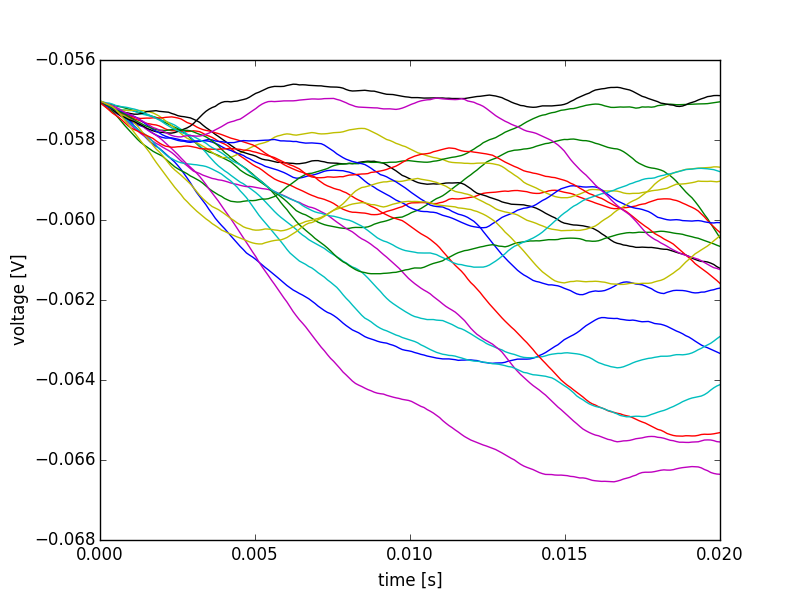
\includegraphics[width=1.0\linewidth]{./Plots/Our_Plots/noise}
  	  		  \caption{}
  	  		  \label{fig:noise}
  	    		
  	    	\end{minipage}
  	    	\hfill
  	    	\begin{minipage}[hbt]{8.4 cm}
  
  	    \centering
  	    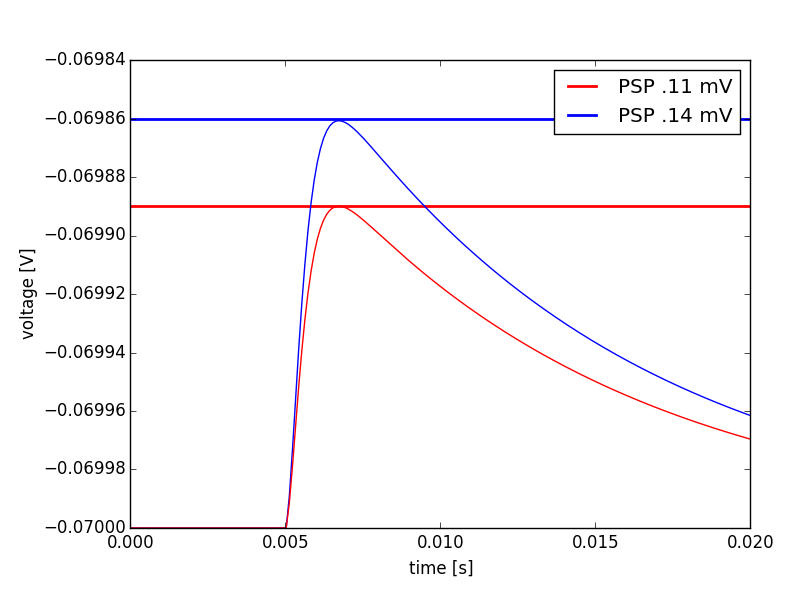
\includegraphics[width=1.0\linewidth]{./Plots/Our_Plots/PSP}
  	    \caption{}
  	    \label{fig:PSP}
  	    	\end{minipage}
  	    	\end{figure}
  
  
  \begin{figure}[H]
  \centering
  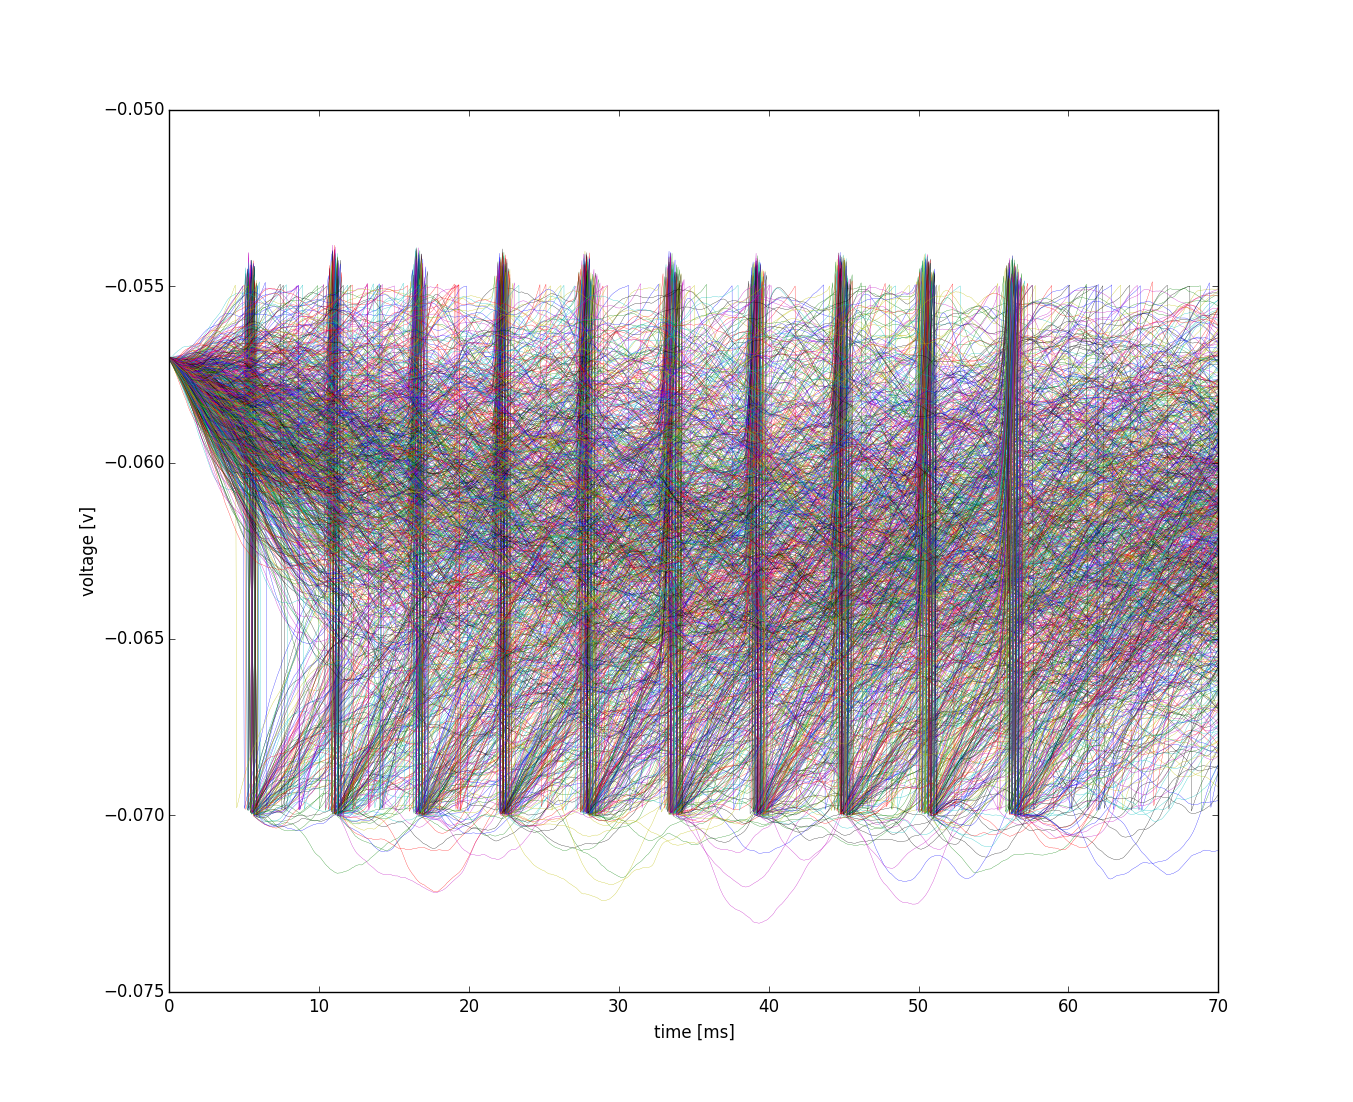
\includegraphics[width=1.0\linewidth]{./Plots/Our_Plots/voltageplot}
  \caption{Voltage traces of all 100 neurons in all of the 10 groups. Clearly visible are the spiking ensembles of the groups and a moderate synchronization process throughout the network. After reaching the threshold at $V_{thresh}=-54.0 mV$ the voltage is resetted to the resting potential $V_{rest}=-70.0 mV$. }
  \label{fig:voltageplot}
  \end{figure}



	\begin{figure}[H]
	    	\begin{minipage}[hbt]{8.2 cm}
	  		\centering
	  		 
	  		  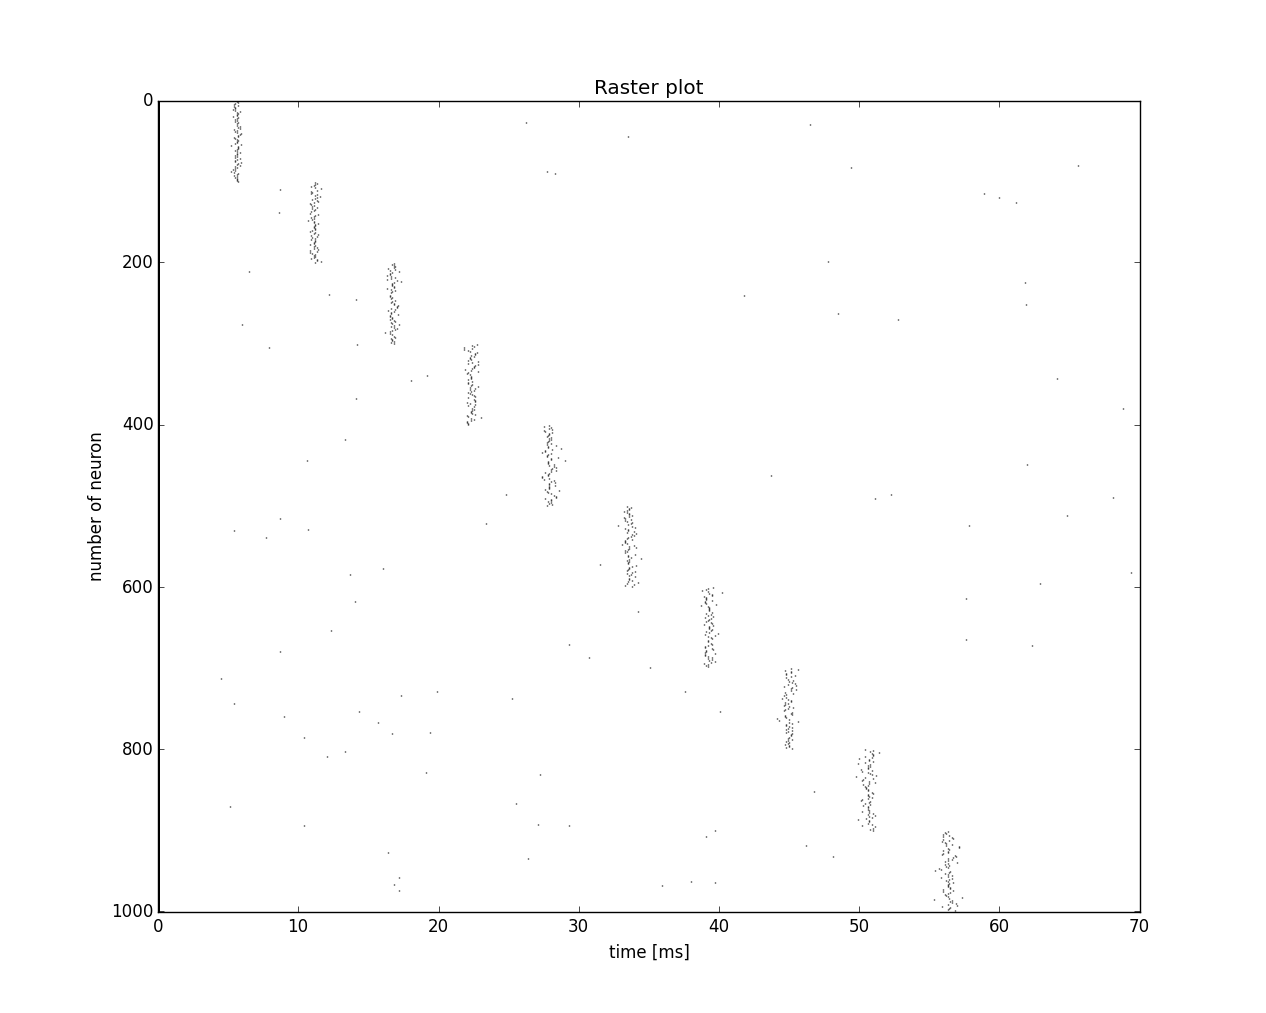
\includegraphics[width=1.0\linewidth]{./Plots/Our_Plots/rasterplot}
	  		  \caption{Synchronization}
	  		  \label{fig:rasterplot}
	    		
	    	\end{minipage}
  	    	\hfill
	    	\begin{minipage}[hbt]{8.2 cm}

	    \centering
	    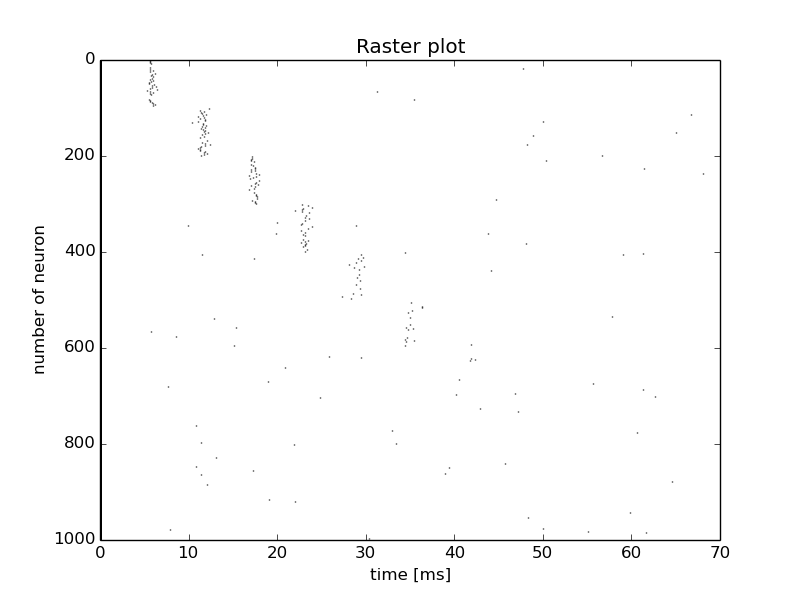
\includegraphics[width=1.0\linewidth]{./Plots/Our_Plots/asynchronization_rasterplot}
	    \caption{Asynchronization}
	    \label{fig:asynchronization_rasterplot}
	    	\end{minipage}
	    	\end{figure}


  \section{Discussion}
         
  \section{Conclusion}
  
  The main conclusion of this project is that information processing via spike timing is indeed possible in spite of the background noise. In most cases the noise does not interfere with the synchronization and even precise synchronous firing is feasible. This allows for an increased information capacity compared to frequency-coded information processing.
  
  For this network which carries information by precise spike timing a relatively large group of neurons is needed. However, neurons can participate in several volleys simultaneously and the network only needs to be locally feedforward.
 

\end{document}